\documentclass{beamer}

%% \documentclass[handout]{beamer}
%% % use this with the [handout] option to create handouts for the audience
%% \usepackage{pgfpages}
%% \pgfpagesuselayout{2 on 1}[a4paper,border shrink=5mm]

\mode<presentation>
{
  \usetheme{Diku}
% set this to your preferences:
  \setbeamercovered{invisible}
%  \setbeamercovered{transparent}
}

\usepackage{graphicx}
\usepackage{epic}

\usepackage{amsmath}
\usepackage{amssymb}
\usepackage{amsthm}

\newcommand{\basetop}[1]{\vtop{\vskip-1ex\hbox{#1}}}
\newcommand{\source}[1]{\let\thefootnote\relax\footnotetext{\scriptsize\textcolor{kugray1}{Source: #1}}}

% for coloured code citation in text:
\usepackage{fancyvrb}

%%%%%%%%%%%%%%%%%%%%%%%%%%%%%%%%%
%%%%%    code sections   %%%%%%%%
%%%%%%%%%%%%%%%%%%%%%%%%%%%%%%%%%

% code highlighting commands in own block
\DefineVerbatimEnvironment{code}{Verbatim}{fontsize=\scriptsize}
\DefineVerbatimEnvironment{icode}{Verbatim}{fontsize=\scriptsize}

% Fancy code with color commands:
\DefineVerbatimEnvironment{colorcode}%
        {Verbatim}{fontsize=\scriptsize,commandchars=\\\{\}}

%%%%%%%%%%%%%%%%%%%%%%%%%%%%%%%%%%
%%%%%    some coloring    %%%%%%%%

\definecolor{Red}{RGB}{220,50,10}
\definecolor{Blue}{RGB}{0,51,102}
\definecolor{Yellow}{RGB}{102,51,0}
\definecolor{Orange}{RGB}{178,36,36}
\definecolor{Grey}{RGB}{180,180,180}
\definecolor{Green}{RGB}{20,120,20}
\definecolor{Purple}{RGB}{160,50,100}
\newcommand{\red}[1]{\textcolor{Red}{{#1}}}
\newcommand{\blue}[1]{\textcolor{Blue}{{#1}}}
\newcommand{\yellow}[1]{\textcolor{Yellow}{{#1}}}
\newcommand{\orange}[1]{\textcolor{Orange}{{#1}}}
\newcommand{\grey}[1]{\textcolor{Grey}{{#1}}}
\newcommand{\green}[1]{\textcolor{Green}{{#1}}}
\newcommand{\purple}[1]{\textcolor{Purple}{{#1}}}




% use "DIKU green" from our color theme for \emph
\renewcommand{\emph}[1]{\textcolor{structure}{#1}}
% use some not-too-bright red for an \emp command
\definecolor{DikuRed}{RGB}{130,50,32}
\newcommand{\emp}[1]{\textcolor{DikuRed}{ #1}}
\definecolor{CosGreen}{RGB}{10,100,70}
\newcommand{\emphh}[1]{\textcolor{CosGreen}{ #1}}
\definecolor{CosBlue}{RGB}{55,111,122}
\newcommand{\emphb}[1]{\textcolor{CosBlue}{ #1}}
\definecolor{CosRed}{RGB}{253,1,1}
\newcommand{\empr}[1]{\textcolor{CosRed}{ #1}}

\newcommand{\mymath}[1]{$ #1 $}
\newcommand{\myindx}[1]{_{#1}}
\newcommand{\myindu}[1]{^{#1}}

\newtheorem{mydef}{Definition}
\newtheorem{mytheo}{Theorem}
\newtheorem{mylemma}{Lemma}


%%%%%%%%%%%%%%%%%%%%

\title[Intro]{Lab 1: A Gentle Introduction to CUDA}

\author[C.~Oancea]{Cosmin E. Oancea\\{\tt cosmin.oancea@diku.dk}\\
\emp{After previous year slides of Rasmus Fonseca!}}

\institute{Department of Computer Science (DIKU)\\University of Copenhagen}


\date[Sept 2017]{September 2017 PMPH Lab Slides}


\begin{document}

\titleslide

%%%%%%%%%%%%%%%%%%%%%%%%%%%%%%%%%%%%%%%%%%%%%%%%%%%
%%%%%%%%%%%%%%%%%%%%%%%%%%%%%%%%%%%%%%%%%%%%%%%%%%%
%%%%%%%%%%%%%%%%%%%%%%%%%%%%%%%%%%%%%%%%%%%%%%%%%%%


\begin{frame}[fragile,t]
\frametitle{Get CUDA Up and Running}

Option 1: Personal computer
\begin{itemize}
    \item \blue{\tt https://developer.nvidia.com/cuda-downloads}
    \item \emp{Don't do this now!}
\end{itemize}

\end{frame}



\begin{frame}[fragile,t]
\frametitle{Get CUDA Up and Running}

Option 2: Using gpu-servers:
\begin{itemize}
    \item {\tt \$ ssh -l <username> ssh-diku-apl.science.ku.dk}
    \item Password:
    \item {\tt \$ ssh gpu01-diku-apl}
    \item Password:
    \item Add the following to your {\tt .bashrc} file:
        \begin{itemize}
            \item {\tt \$ export PATH=/usr/local/cuda/bin:\$PATH}
            \item {\tt \$ export LD\_LIBRARY\_PATH=/usr/local/cuda/lib64:\$LD\_LIBRARY\_PATH}
            \item {\tt \$ export LIBRARY\_PATH=\$LD\_LIBRARY\_PATH:\$LIBRARY\_PATH}
        \end{itemize}
    \item And you are ready to go:\\{\tt \$ nvcc ... }
\end{itemize}

\end{frame}

%\begin{frame}[fragile,t]
%\frametitle{Setting up No-Password SSH}
%
%\emp{On your local machine, add an entry in {\tt .ssh/config}\\ for each gpu01..4:}\\
%\medskip
%
%\begin{scriptsize}
%{\tt Host gpu01-diku-apl}\\
%{\tt ProxyCommand ssh -q <user-name>@ssh-diku-apl.science.ku.dk nc -q0 gpu01-diku-apl 22}\\
%{\tt user <user-name>}
%\end{scriptsize}
%\bigskip
%
%\emp{On each gpu server copy-past your local-machine {\tt id\_rsa.pub} into
%the {\tt .ssh/authorized\_keys} file.}
%
%\medskip
%
%Now you should be able to log in from your local machine with:\\
%{\tt\$ ssh gpu01-diku-apl}
%
%\end{frame}


\begin{frame}[fragile,t]
\frametitle{Let's Try it Out:}

{\tt \$ ssh gpu01}\medskip\\
{\tt \$ cp -r /usr/local/cuda/samples .}\medskip\\
{\tt \$ cd samples/1\_Utilities/deviceQuery}\medskip\\
{\tt \$ make}\medskip\\
{\tt \$ ./deviceQuery}\medskip\\

\end{frame}

\begin{frame}[fragile,t]
\frametitle{GPU Programming Online Courses}

www.udacity.com/course/cs344

\end{frame}

\begin{frame}[fragile,t]
\frametitle{Motivation for Using GPGPUs}

\begin{center}
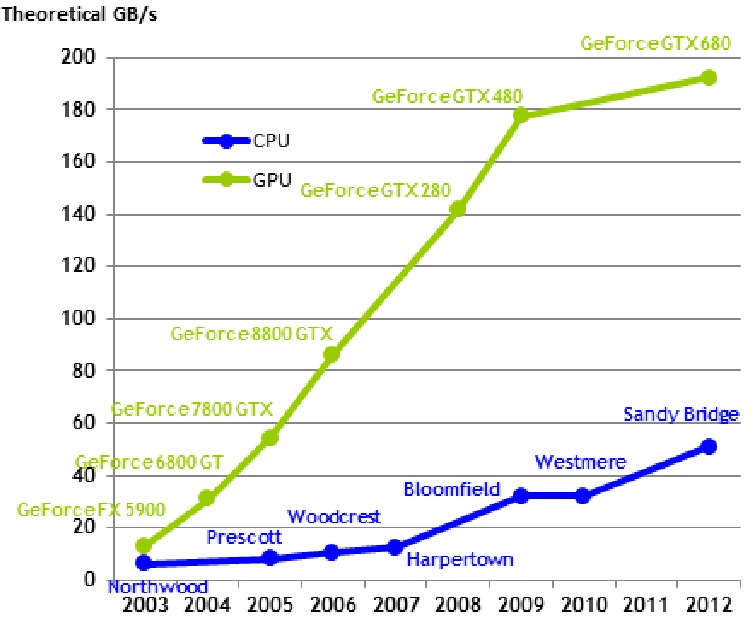
\includegraphics[height=45ex]{Figures/Lab1/Bandwidth.png}
\end  {center}

\end{frame}

\begin{frame}[fragile,t]
\frametitle{Motivation for Using GPGPUs}

\begin{center}
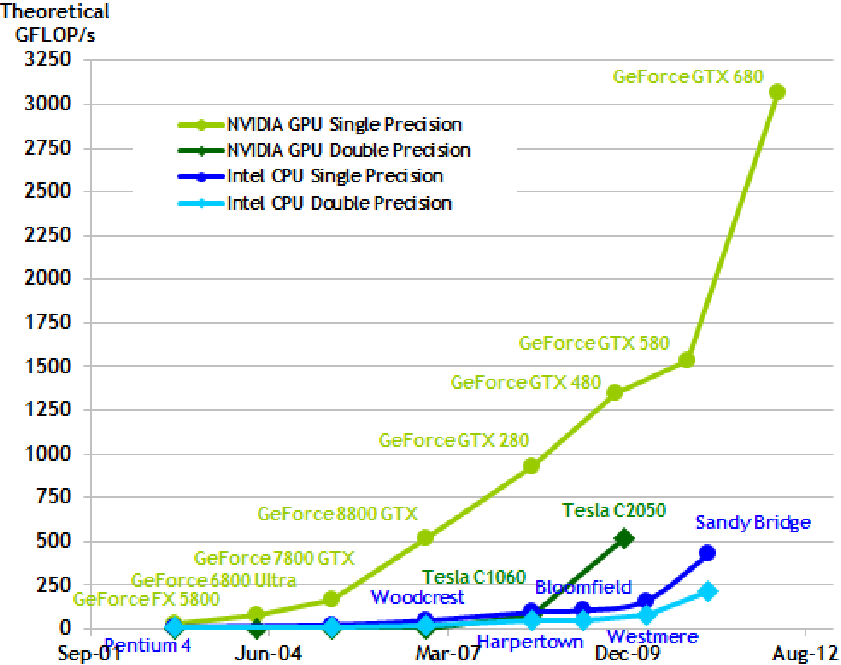
\includegraphics[height=43ex]{Figures/Lab1/GFlops.png}
\end  {center}

\end{frame}

\begin{frame}[fragile,t]
\frametitle{Difficulties in Programming GPGPUs}

\begin{center}
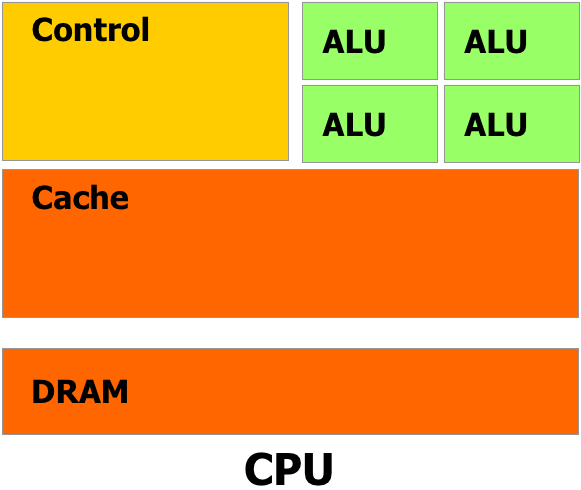
\includegraphics[height=24ex]{Figures/Lab1/MulticoreArch.png}$\mbox{ }\mbox{ }\mbox{ }$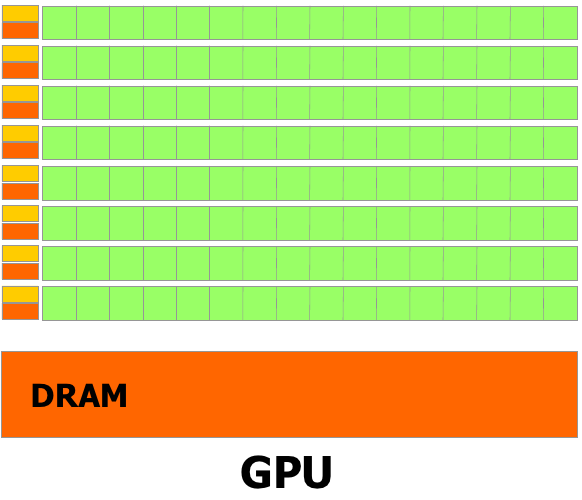
\includegraphics[height=25ex]{Figures/Lab1/GPGPUarch.png}
\end  {center}


\end{frame}



\begin{frame}[fragile,t]
\frametitle{GPGPU programming}

\begin{center}
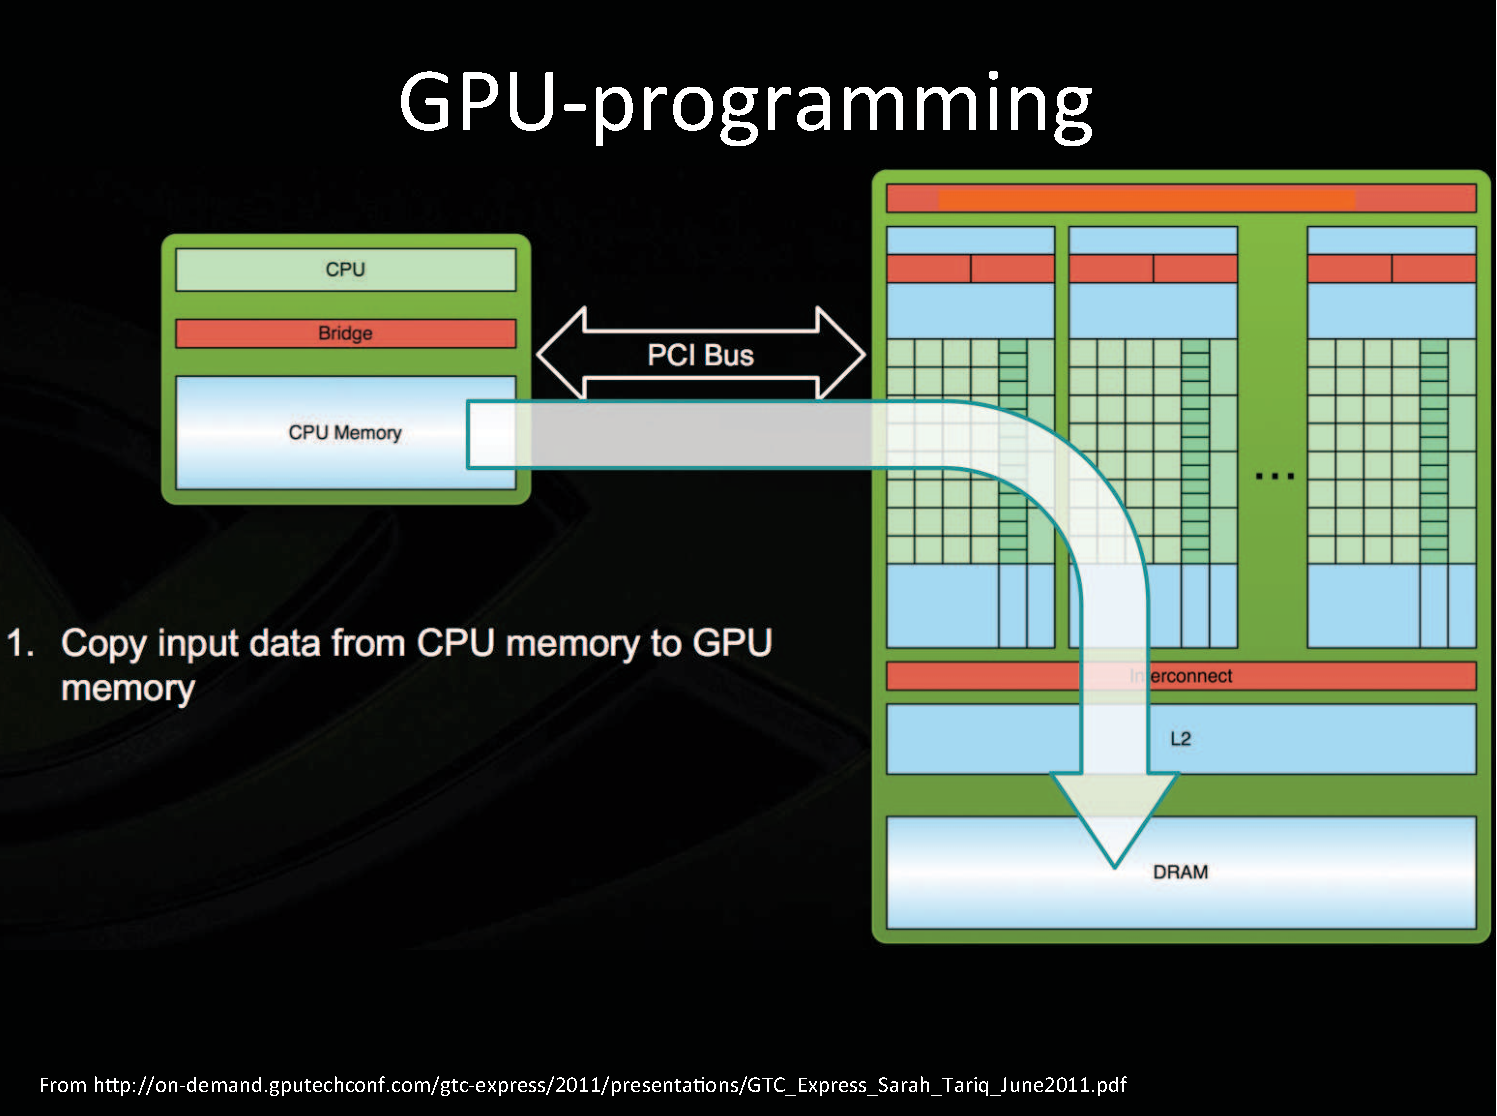
\includegraphics[height=43ex]{Figures/Lab1/MemCpy1.pdf}
\end  {center}

\end{frame}

\begin{frame}[fragile,t]
\frametitle{GPGPU programming}

\begin{center}
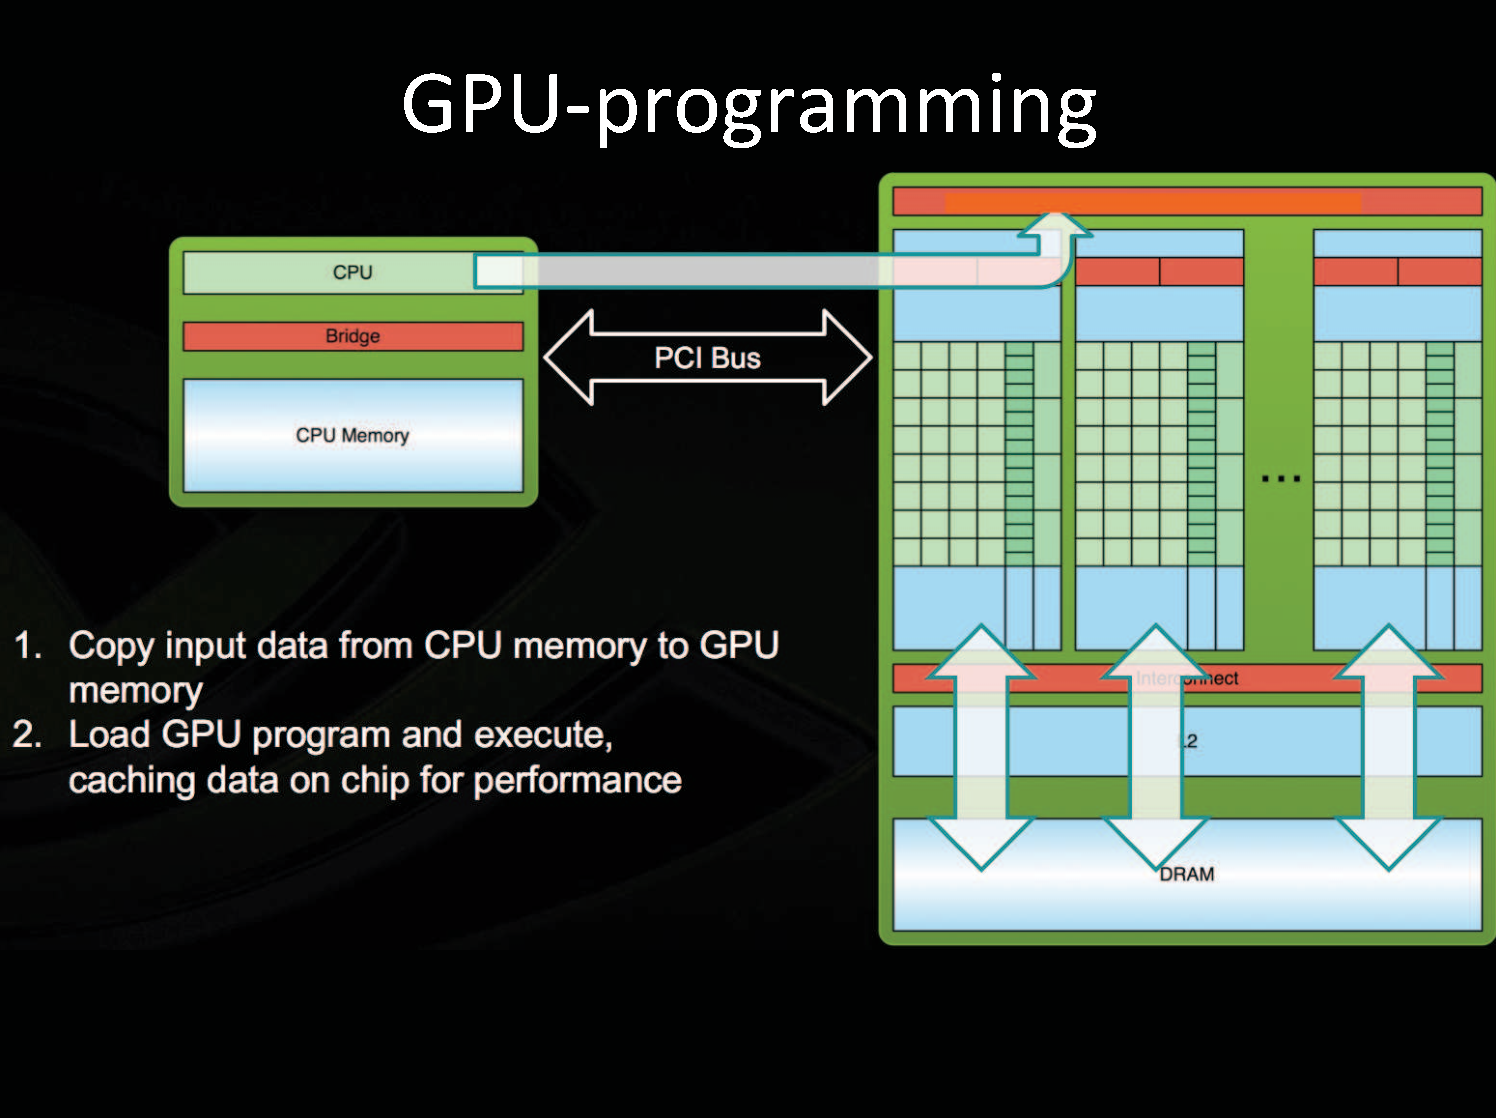
\includegraphics[height=43ex]{Figures/Lab1/MemCpy2.pdf}
\end  {center}

\end{frame}


\begin{frame}[fragile,t]
\frametitle{GPGPU programming}

\begin{center}
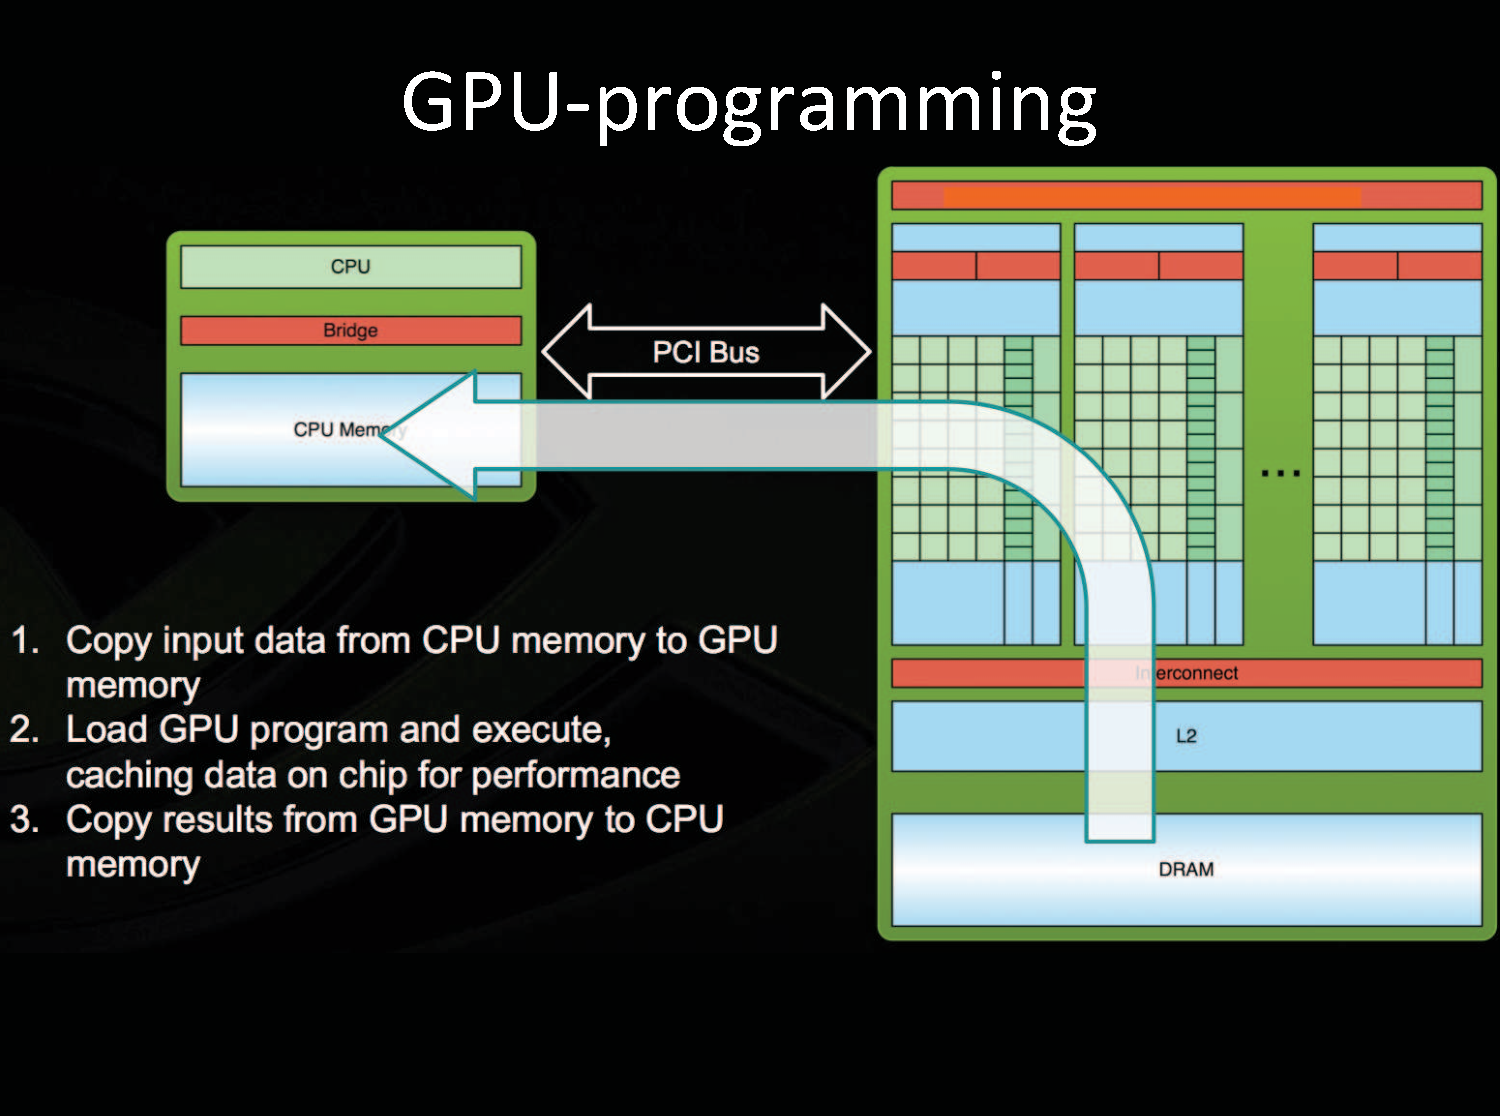
\includegraphics[height=43ex]{Figures/Lab1/MemCpy3.pdf}
\end  {center}

\end{frame}


\begin{frame}[fragile,t]
\frametitle{GPGPU programming}

\begin{center}
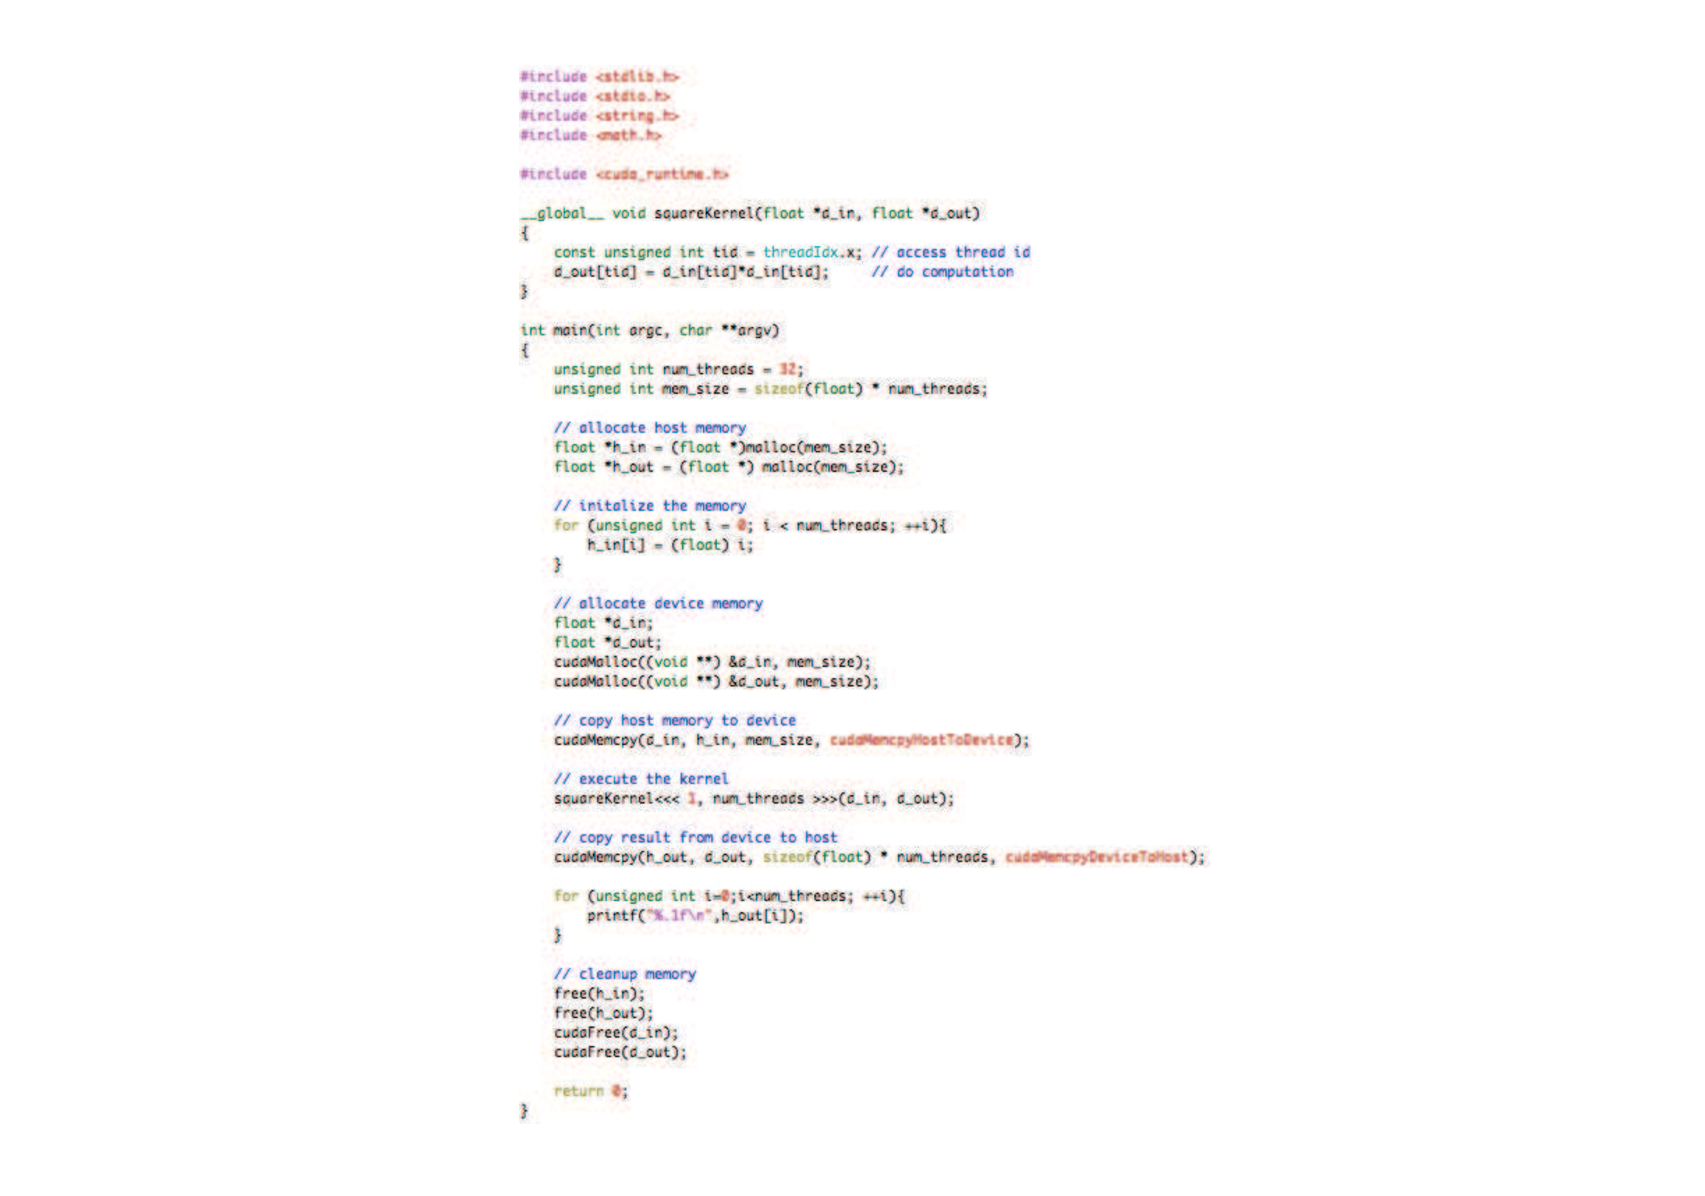
\includegraphics[height=43ex]{Figures/Lab1/CUDAsimple.pdf}
\end  {center}

\end{frame}


\begin{frame}[fragile,t]
\frametitle{A Simple CUDA Program}

\begin{colorcode}[fontsize=\scriptsize]
#include <stdlib.h>
#include <stdio.h>
#include <string.h>
#include <math.h>
#include <cuda_runtime.h>

\emp{__global__ void squareKernel(float* d_in, float *d_out) \{}
\emp{    const unsigned int lid = threadIdx.x;} \blue{// local id inside a block}
\emp{    const unsigned int gid = blockIdx.x*blockDim.x + lid;} \blue{// global id}
\emp{    d_out[gid] = d_in[gid]*d_in[gid];}     \blue{// do computation}
\emp{\}}

int main(int argc, char** argv) \{
    unsigned int num_threads = 32;
    unsigned int mem_size    = num_threads*sizeof(float);

    \blue{// allocate host memory}
    float* h_in  = (float*) malloc(mem_size);
    float* h_out = (float*) malloc(mem_size);

    \blue{// initialize the memory}
    for(unsigned int i=0; i<num_threads; ++i)\{
        h_in[i] = (float)i;
    \}
\end{colorcode}
\end{frame}

\begin{frame}[fragile,t]
\frametitle{A Simple CUDA Program (continuation)}
\begin{colorcode}[fontsize=\scriptsize]
    \blue{// allocate device memory}
    float* d_in;
    float* d_out;
    cudaMalloc((void**)&d_in,  mem_size);
    cudaMalloc((void**)&d_out, mem_size);

    \blue{// copy host memory to device}
    cudaMemcpy(d_in, h_in, mem_size, cudaMemcpyHostToDevice);

    \blue{// execute the kernel}
    squareKernel<<< 1, num_threads>>>(d_in, d_out);

    \blue{// copy result from ddevice to host}
    cudaMemcpy(h_out, d_out, sizeof(float)*num_threads, cudaMemcpyDeviceToHost);

    \blue{// print result}
    for(unsigned int i=0; i<num_threads; ++i) printf("\%.6f\mymath{\backslash}n", h_out[i]);

    // clean-up memory
    free(h_in);       free(h_out);
    cudaFree(d_in);   cudaFree(d_out);   
\}
\end{colorcode}
\end{frame}


\begin{frame}[fragile,t]
\frametitle{Save, Compile, Run}
{\tt \$ nvcc -O3 simpleCUDA.cu}\\
\bigskip

{\tt \$ ./a.out}
\end{frame}


\begin{frame}[fragile,t]
\frametitle{Measuring Runtime}
\vspace{-2ex}
\begin{colorcode}[fontsize=\scriptsize]
#include <sys/time.h>
#include <time.h>
int timeval_subtract(   struct timeval* result,
                        struct timeval* t2,struct timeval* t1) \{
    unsigned int resolution=1000000;
    long int diff = (t2->tv_usec + resolution * t2->tv_sec) - 
                    (t1->tv_usec + resolution * t1->tv_sec) ;
    result->tv_sec = diff / resolution;
    result->tv_usec = diff \% resolution;
    return (diff<0);
\}
int main() \{ ...
    unsigned long int elapsed;
    struct timeval t_start, t_end, t_diff;
    gettimeofday(&t_start, NULL);

    \blue{// execute the kernel}
    squareKernel<<< 1, num_threads>>>(d_in, d_out);
    \emp{cudaThreadSynchronize();}

    gettimeofday(&t_end, NULL);
    timeval_subtract(&t_diff, &t_end, &t_start);
    elapsed = t_diff.tv_sec*1e6+t_diff.tv_usec;
    printf("Took \%d microseconds (\%.2fms)\mymath{\backslash}n",elapsed,elapsed/1000.0);
...\}
\end{colorcode}
\end{frame}


\begin{frame}[fragile,t]
\frametitle{Trouble Ahead}

This week assignment:\\
{\em Write a CUDA program that maps the function
{\tt (x/(x-2))\^6} to the array {\tt [0,1,..., 32756]} and writes the result
to a file}

\bigskip

This shouldn't be a problem given the shown program 
            (just adapt the kernel a bit), except that:
\begin{itemize}
    \item except that CUDA won't accept a block of size $32757$
        \begin{itemize}
            \item a \emp{\em CUDA warp} is formed by 32 threads that execute in SIMD fashion.
            \item a \emp{\em CUDA block} contains a multiple of $32$ number of threads 
                    (and less than $1024$).  Synchronization is possible inside a
                    CUDA block by means of barrier.
            \item Barrier synchronization is not possible outside the CUDA block
                    (only by finishing the kernel)!
        \end{itemize}
    \item furthermore if the size of the computation does not exactly matches
            a multiple of block size, then you need to spawn extra threads, but
            add an {\tt if} inside the kernel so that the extra threads do no work!
\end{itemize}
\end{frame}

\begin{frame}[fragile,t]
\frametitle{GPGPU in More Detail}

\begin{center}
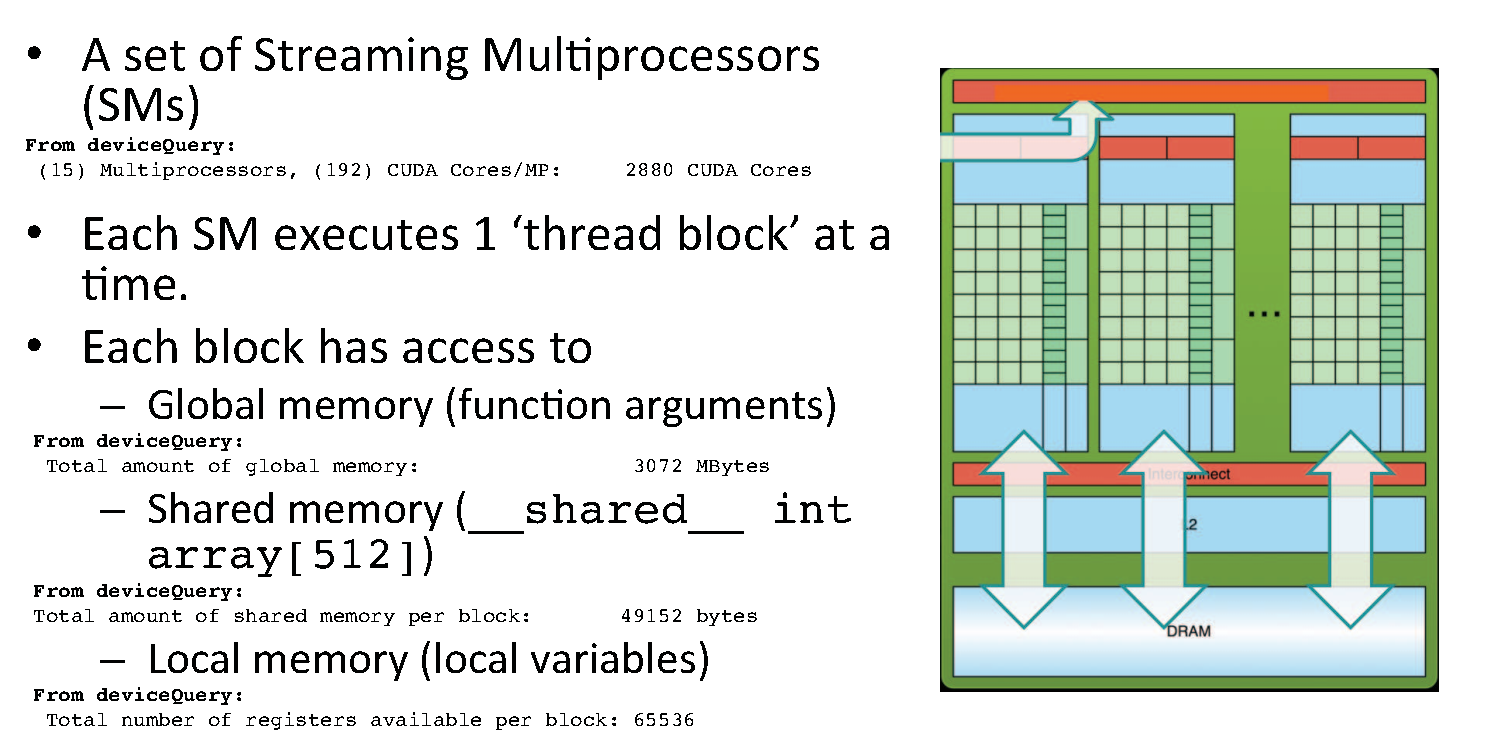
\includegraphics[height=35ex]{Figures/Lab1/GPUorg.pdf}
\end  {center}

\end{frame}


\begin{frame}[fragile,t]
\frametitle{Running Multiple Blocks}
\begin{colorcode}[fontsize=\scriptsize]

    unsigned int num_threads = 32757;
    unsigned int mem_size    = num_threads*sizeof(float);
    unsigned int block_size  = 256;
    unsigned int num_blocks  = ((num_threads + (block_size - 1)) / block_size);

    \blue{// execute the kernel}
    squareKernel<<< num_blocks, block_size>>>(d_in, d_out, num_threads);

...

\emp{__global__ void squareKernel(float* d_in, float *d_out, int threads_num) \{}
\emp{    const unsigned int lid = threadIdx.x;} \blue{// local id inside a block}
\emp{    const unsigned int gid = blockIdx.x*blockDim.x + lid;} \blue{// global id}
    if(gid < threads_num) \{
    \emp{    d_out[gid] = d_in[gid]*d_in[gid];}     \blue{// do computation}
    \emp{\}}
\emp{\}}
\end{colorcode}
\end{frame}


\end{document}
